\section{Introduction}

The recent rapid advancement of artificial intelligence is largely driven by the success of
Transformer models~\cite{attention-is-all-you-need,bert,gpt3}, which revolutionize applications
ranging from language translation, text generation~\cite{chatgpt}, image recognition~\cite{vit},
to autonomous driving~\cite{transformer-autonomous}.
Due to their enormous computational demands~\cite{energy-scaling-laws},
Transformer models are typically run on specialized hardware accelerators to
achieve practical performance and energy efficiency.
As these models continue to scale in size and complexity~\cite{scaling-laws},
the need for efficient hardware acceleration becomes increasingly critical.

\begin{figure}[t]
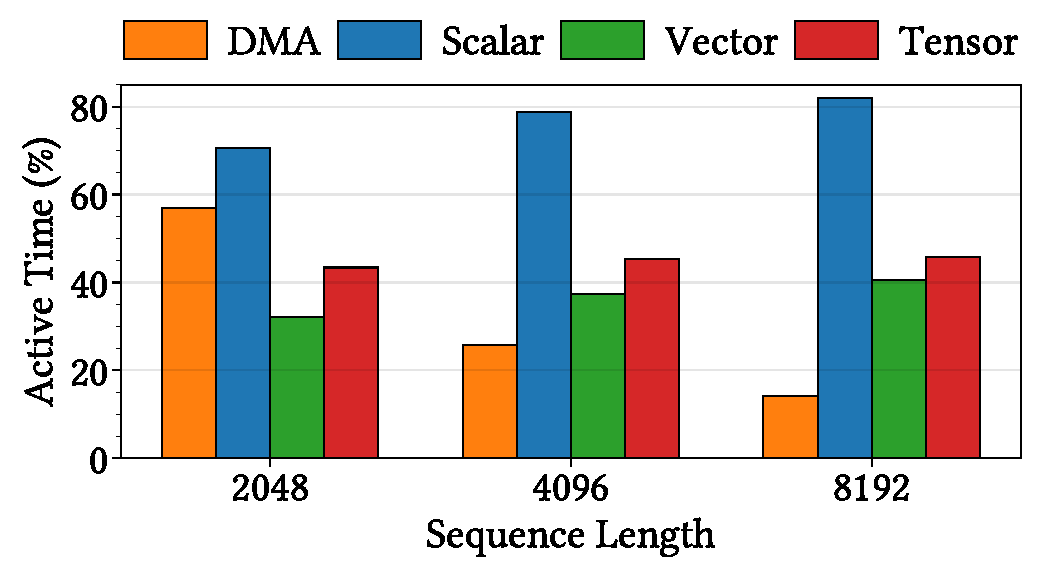
\includegraphics[width=1.0\columnwidth]{figure_src/active_time.pdf}
\caption{Percentage of active time of various components in AWS NeuronCore-v2 when running \FA{}.}
\label{fig:aws-active-time}
\Description{Active Time}
\end{figure}

Systolic arrays~\cite{original_systolic} are widely used in both industry~\cite{google-tpu-arch,tpuv1,tpuv4,trainium-arch} and
academic accelerators~\cite{ucb-gemmini} to run deep learning workloads.
In systolic arrays, data is continuously streamed through a network of tightly coupled processing elements (PEs) to
maximize computation density while minimizing data movement overhead.
Despite various dataflows~\cite{eyeriss-jssc,eyeriss-isca,flat,fusemax} proposed for systolic arrays,
the multiply-accumulate (MAC)-based two-dimensional (2D) systolic array is most widely adopted,
as in Google's TPU~\cite{google-tpu-arch,tpuv1,tpuv4} and AWS NeuronCore~\cite{trainium-arch} that are mostly deployed for running Transformer models.

The key operation in Transformer models is the \emph{scaled dot-product attention} (SDPA),
which is usually implemented using the \emph{\FA{}}~\cite{fa2,fa3} algorithm.
When running \FA{} on systolic-array-based accelerators, matrix multiplications are executed on the systolic array,
while softmax operations are offloaded to external vector and scalar units.
The reliance on this simplistic division of labor forces vector/scalar units to supply adequate
floating-point operations per second (\FLOPs{}) for softmax,
failing to do so causes them to bottleneck the overall pipeline.
As shown in \autoref{fig:aws-active-time}, when running \FA{} on AWS NeuronCore-v2,
the systolic array (tensor engine) is only active for about 45\% of the time, while the scalar units remain 
active for 80\% of the time.

The simplistic mapping of computation also creates another source of low hardware utilization:
as \FA{} computes softmax between two matrix multiplications, data must be transferred
back and forth frequently between the systolic array and vector/scalar units through a local SRAM,
thereby preventing reuse of any matrix data across iterations,
increasing preloading overhead, and exacerbating SRAM port contention~\cite{virgo,mosaic}.
As shown in our experiments in \autoref{sec:eval-performance}, the 
systolic array of AWS NeuronCore-v2 only achieves 25\% of the
theoretical \FLOPs{} utilization, even though it is active for 45\% of the time.

We argue that the above performance problems can be addressed by running the entire \FA{}
solely on the systolic array, where matrix multiplications and softmax can utilize and share the systolic array \FLOPs{} at a finer granularity.
As a result, softmax is no longer limited by the throughput of vector/scalar units, and both
data movement overhead and SRAM port contention are eliminated as all computations occur at the same place.
To efficiently implement this approach, apart from executing softmax operations, including \texttt{exp}, \texttt{rowmax}, and \texttt{rowsum},
using only the systolic array, various operations must also be effectively overlapped to maximize array utilization.
FuseMax~\cite{fusemax} pioneered the efficient fusion of \FA{} on systolic arrays.
While it addresses the challenge of handling softmax by mapping \texttt{rowmax} and \texttt{rowsum} as spatial reductions,
its core strategy for achieving high hardware utilization is to process multiple \FA{} iterations simultaneously.
This parallel processing approach, however, necessitates storing multiple contexts inside each PE to enable context switching
among iterations, leading to additional hardware overhead.

We propose \emph{\MSAGA{}}, a new hardware-friendly systolic array architecture that
fully unleashes the performance potential of systolic arrays by running the entire \FA{}
on a single systolic array with minimal area overhead.
\MSAGA{} regards \texttt{rowmax} and \texttt{rowsum} as reduction operations and
performs them on-the-fly and in-place with an array of comparators and a specialized upward data path, thereby eliminating the
need to store them in local SRAM.
To calculate \texttt{exp}, \MSAGA{} reuses the systolic array to perform linear interpolation~\cite{exp_pwl}
to approximate the result, taking advantage of the fact that the input of \texttt{exp} is always less than or equal to zero.
Based on \MSAGA{}, we also introduce \emph{\SA{}},
an optimized kernel that makes the best use of \MSAGA{}'s capabilities to overlap
multiple operations within the same \FA{} iteration,
further improving array utilization while preserving the
order of all floating-point operations in \FA{}.

We make the following contributions in this paper:
\begin{itemize}
    \item
    We propose \MSAGA{}, an enhanced systolic array architecture that can execute the
    entire \FA{} solely on the systolic array without any vector or scalar units.
    We implement \MSAGA{} in synthesizable RTL, achieving clock frequency of 1.5\,GHz
    under 16\,nm technology.
    Our synthesis result shows that \MSAGA{} only incurs 12\% additional area overhead
    compared to the baseline systolic array.

    \item 
    We propose \SA{}, an optimized kernel for \MSAGA{} to efficiently overlap operations inside a single \FA{} iteration.
    With \SA{}, \MSAGA{} achieves 1.77$\times$ and 4.83$\times$ higher \FLOPs{} utilization
    than AWS NeuronCore-v2 and TPUv5e, respectively.

    \item
    We develop a Python programming interface that allows users to write custom kernels for \MSAGA{}.
    We open-source both the RTL implementation and the Python software stack at \MSAGAURL{}.
\end{itemize}

